%%%%%%%%%%%%%%%%%%%%%%%%%%%%%%%%%%%%%%%%%%%%%%%%%%%%%%%%%%%%%%%%%%%%%%%%
% Plantilla TFG/TFM
% Universidad de A Coruña. Facultad de Informática
% Realizado por: Welton Vieira dos Santos
% Modificado: Welton Vieira dos Santos
% Contacto: welton.dossantos@udc.es
%%%%%%%%%%%%%%%%%%%%%%%%%%%%%%%%%%%%%%%%%%%%%%%%%%%%%%%%%%%%%%%%%%%%%%%%


\chapter{Desarrollo técnico}
\section{Videojuego en 2D}
\subsection{Descripción}ISS Manticore es un scroll lateral con ligeros tintes de metroidvania\footnote{Metroidvania: es un subgénero de juego basado en un concepto de plataformas no lineal con un mundo conectado que fomenta que el jugador lo explore} en el diseño de escenarios al tener algunos incentivos para desviarse del camino principal, pero dividido en niveles donde los jugadores comienzan cada fase en el extremo izquierdo de un escenario lineal.

Su objetivo es alcanzar la salida de la nave de la cual se ha quedado atrapado en el momento que ha intentado entregar un paquete en la misma.

El protagonista va avanzando y derrotando los enemigos que contiene en cada fase.
\subsection{Personajes}
Jackie, el protagonista del juego tendrá que completar distintas fases, en las que tendrá que superar distintos enemigos y acometer distintas tareas para alcanzar su objetivo, para ello el jugador tendrá que mover al protagonista empleando las flechas del teclado para avanzar, esquivar a los enemigos y recoger los coleccionables necesarios y disparando con un click de ratón a los distintos personajes que se interpongan en su camino.

\subsection{Enemigos}
Los enemigos se interponen en el camino del protagonista habitando los diferentes escenarios por los que avanza dañando al protagonista si este entra en contacto con los enemigos. 
\begin{itemize}
    \item \textbf{Octopus:} Estos pequeños seres extraños se encuentran levitando en una misma posición con el objetivo de interrumpir al protagonista en su camino para completar su cometido. Ejemplo en la Figura \ref{fig:Octopus}.
    \item \textbf{Tortugas:} Están en constante movimiento de un lado a otro y dificultan el transcurso del personaje, que debe abatirlos o esquivarlos, para no salir dañado y conseguir completar su misión. Ejemplo en la Figura \ref{fig:Tortuga}.
    \item \textbf{Spiderbots:} Son el enemigo más difícil de derrotar para el protagonista debido a que dispara proyectiles cada 10 segundos que pueden dañarlo si no es capaz de esquivarlos. Ejemplo en la Figura \ref{fig:Octopus}. 
\end{itemize}

\subsection{Diseño}
\subsubsection{Patrón estrategia}
Este patrón ha sido utilizado en la gran mayoría del código, con la idea de abstraer en clases una serie de estados y comportamientos y, a medida que se se van extendiendo otras clases de una forma bastante jerárquica, haciendo que el comportamiento sea cada vez más específico, por ejemplo el Menu principal del juego que está compuesto por varios componentes como imágenes, botones (estilo rolover) para seleccionar las opciones pertinentes.

\subsubsection{Patrón Singleton}
El patrón singleton está presente en la clase Director, GestorRecursos y tambien en las factorías de los personajes y de las fases del juego. Además de solamente permitir que se instancia solamente un objecto con el uso de clases internas en el caso del director, que solamente tiene uno en todo el proceso.

\subsubsection{Personajes}
La implementación de los personajes hereda de la clase MiSprite y va jerarquizando como se muestra en la Figura \ref{fig:Personaje}. Esa clase incorpora los elementos necesarios para almacenar las posiciones, sprites, velocidades y todos los elementos comunes como el scroll.

\begin{figure}[H]
	\centering
	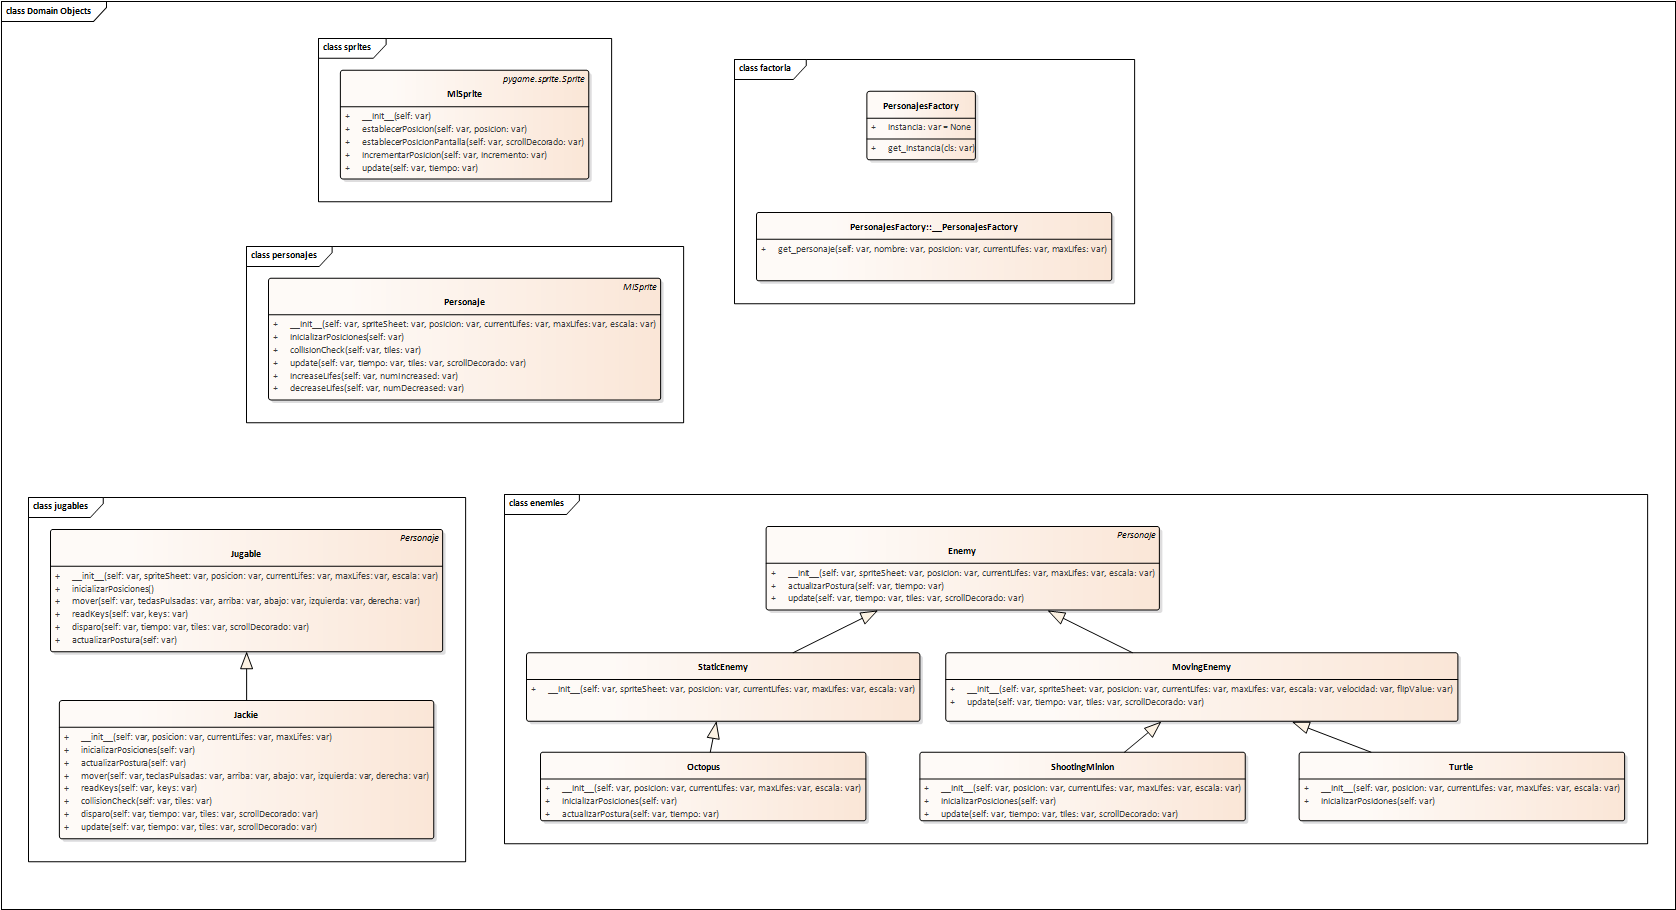
\includegraphics[scale=0.30]{imagenes/Personaje.png}
	\caption{\label{fig:Personaje}Ejemplo de la jerarquía de la clase Personaje}
\end{figure}

Cada objeto del tipo personaje es instanciado por su factoría correspondiente con la intención de permitir un mejor mantenimiento y expansión del código futuramente.

Esos personajes están diferenciados por dos tipos básicos, uno jugable y otro los enemigos.

\subsubsection{Fases}
La implementación de la dinámica de fases es muy similar a la dinámica de los personajes como se puede apreciar en la Figura \ref{fig:Fases} concervando los métodos ``update'', ``eventos'' y ``dibujar'' de la clase Escena.

\begin{figure}[H]
	\centering
	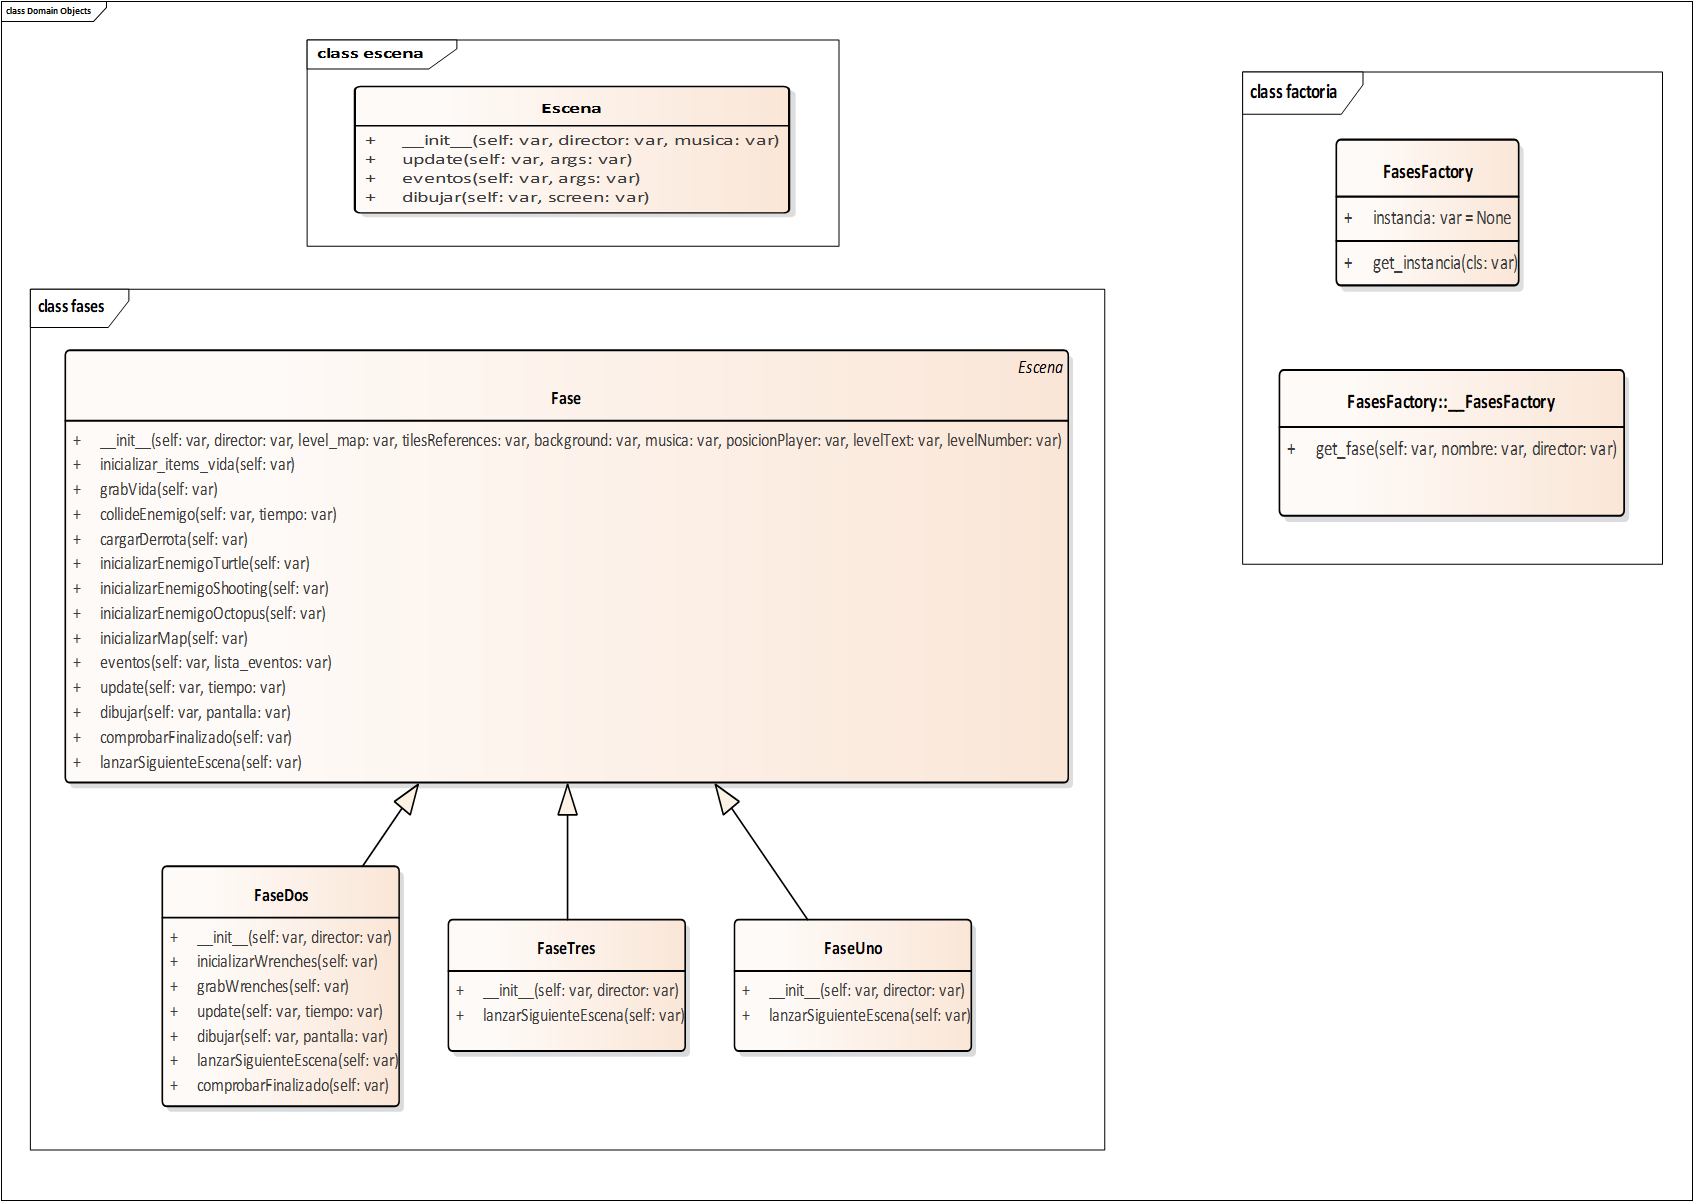
\includegraphics[scale=0.30]{imagenes/Fases.png}
	\caption{\label{fig:Fases}Ejemplo de la jerarquía de la clase Fase}
\end{figure}

\subsubsection{Escena}
La clase Escena define toda las estructura visual del juego, donde desde ahí se puede controlar los menus, personajes, transiciones y etc.

La clase Escena posee tres métodos principales:
\begin{itemize}
	\item eventos: Encargado de leer los eventos producidos por la interacción del usuario con el sistema.
	\item update: Encargado de actualizar el modelo de escena en cuestión basado en los eventos producidos durante la interacción del usuario.
	\item dibujar: Encargado de dibujar los elementos de la parte visual del juego.
\end{itemize}

\subsubsection{Director}
El director es el encargado de ejecutar la escena pertinente, que puede ser un menú o las fases correspondientes de las determinadas etapas del juego. La Figura \ref{fig:Director} muestra su estructura.

\begin{figure}[H]
	\centering
	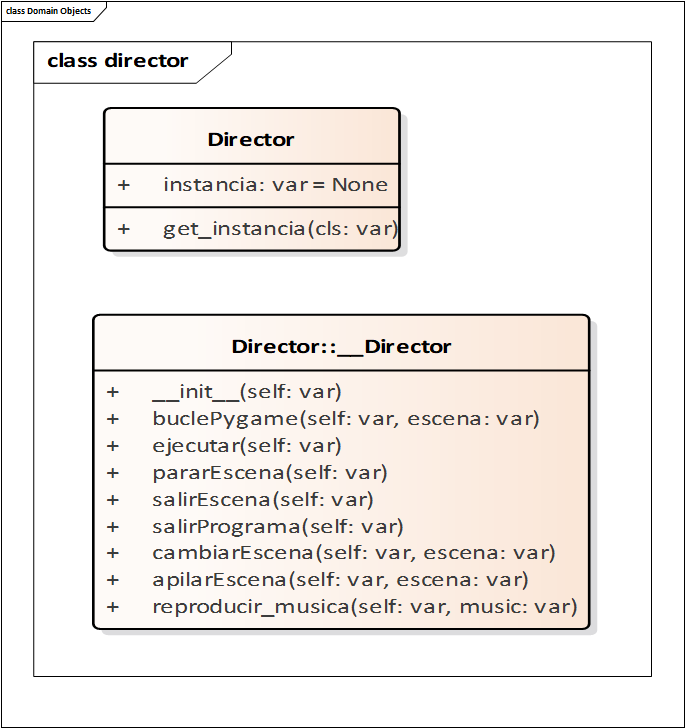
\includegraphics[scale=0.30]{imagenes/Director.png}
	\caption{\label{fig:Director}Ejemplo de la jerarquía de la clase Director}
\end{figure}

Como se puede observar, director possee una clase interna.

\subsubsection{Gestor de recursos}
Como su propio nombre dice, es el encargado de suministrar los recursos necesarios para la una buena interacción con el juego. La Figura \ref{fig:GestorRecursos}

\begin{figure}[H]
	\centering
	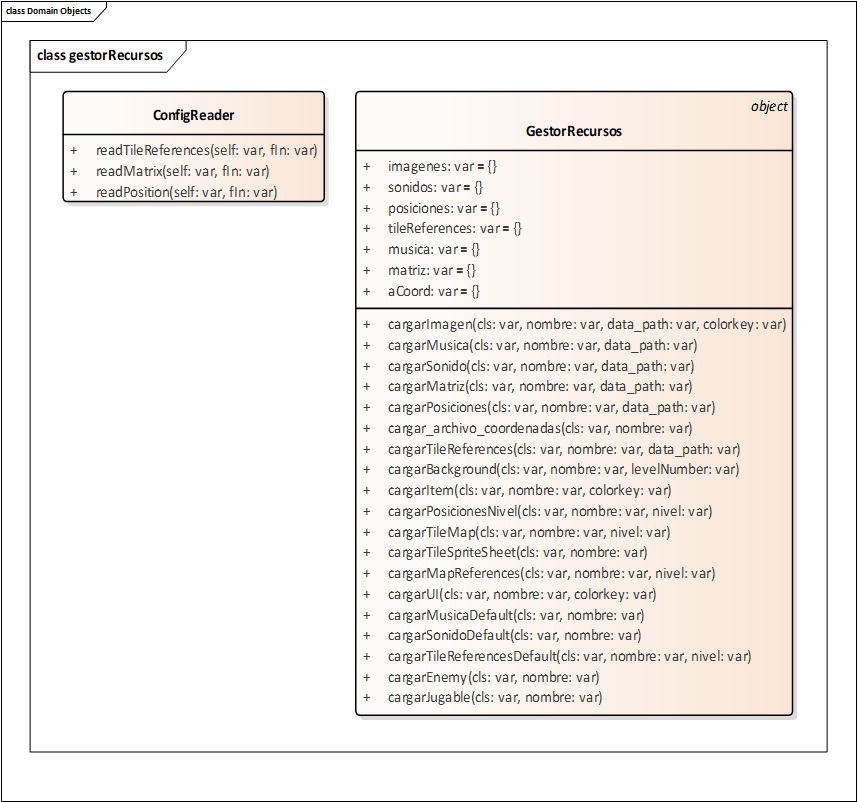
\includegraphics[scale=0.30]{imagenes/GestorRecursos.png}
	\caption{\label{fig:GestorRecursos}Ejemplo uml del gerenciador de recursos}
\end{figure}

\subsection{Escenas}

La transición entre escenas se muestra en el diagrama de la Figura \ref{fig:TrasicionEscenas}. 

\begin{figure}[H]
	\centering
	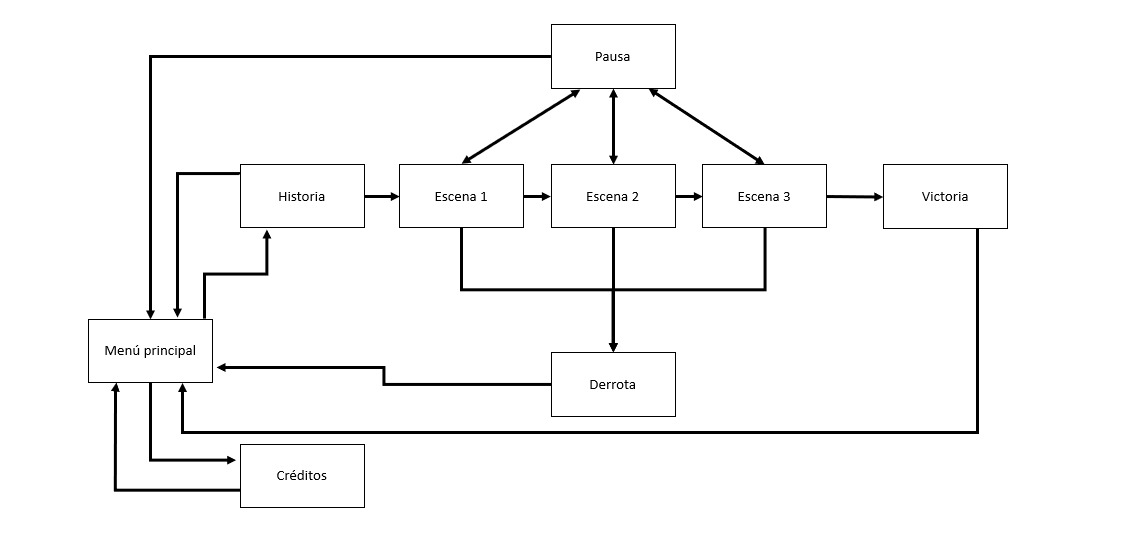
\includegraphics[scale=0.35]{imagenes/transicionEscenas.jpeg}
	\caption{\label{fig:TrasicionEscenas}Diagrama de transición de las escenas}
\end{figure}

\subsubsection{Menú principal}
En esta primera pantalla (Figura \ref{fig:EjemploMenuPrincipal}), que se muestra al jugador nada más ejecutar el juego, se le permite elegir entre comenzar con la historia, visualizar los créditos, lo que enviaría al usuario a la pantalla de Créditos, o la opción de salir, que cerraría el juego. 

\begin{figure}[H]
	\centering
	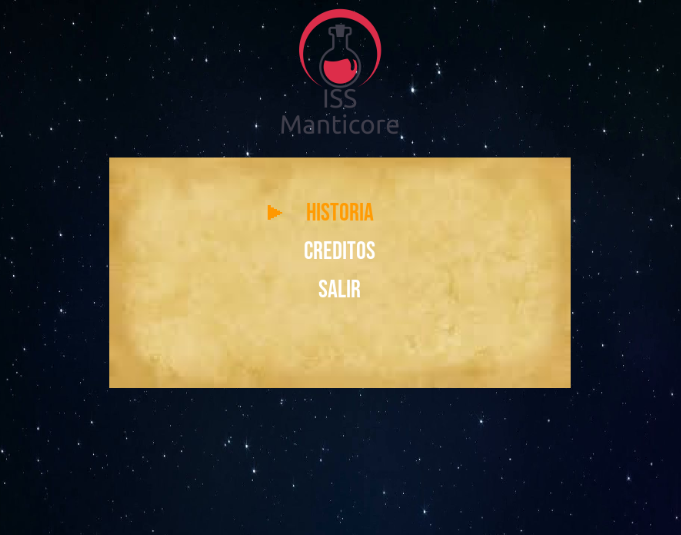
\includegraphics[scale=0.50]{imagenes/EjemploMenuPrincipal.png}
	\caption{\label{fig:EjemploMenuPrincipal}Ejemplo del menu principal}
\end{figure}

\subsubsection{Historia}
Esta pantalla (Figura \ref{fig:EjemploMenuHistoria})muestra un breve resumen de la historia y la leyenda del juego, en la que se puede ver la configuración inicial que contiene la imagen del personaje, el número de vidas inicial, el número de proyectiles con el que cuenta antes de comenzar la aventura (con miras a añadir más adelante objetos de munición y diferentes armas o proyectiles). Desde esta pantalla se puede volver al Menú principal pulsando la tecla Esc o pasar a la Escena 1 pulsando la tecla Enter. 

\begin{figure}[H]
	\centering
	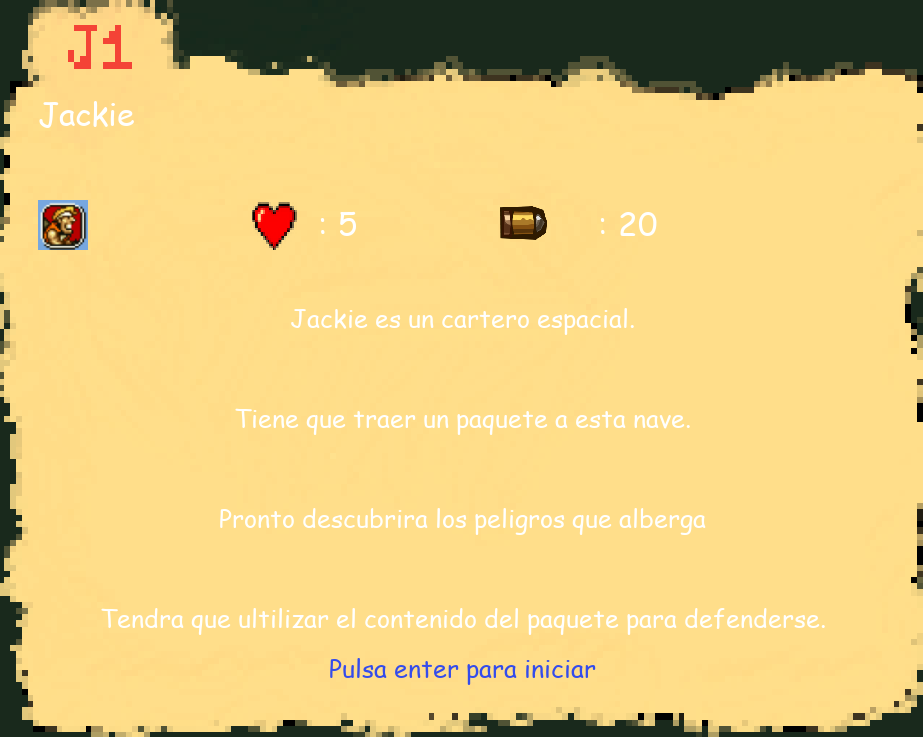
\includegraphics[scale=0.50]{imagenes/EjemploMenuHistoria.png}
	\caption{\label{fig:EjemploMenuHistoria}Ejemplo del apartado historia del menu principal}
\end{figure}

\subsubsection{Fase 1 - Sala de calderas}
La escena comienza con el protagonista en la sala de calderas, este emprende su aventura con tres vidas, que podrá aumentar o disminuir segundo se desenvuelva, nada más arrancar aparece el primer enemigo, un spiderbot al que tendremos que derrotar, si seguimos avanzando nos encontramos con el segundo enemigo, en este caso un octopus, y también con el primer botiquín, que nos permitirá ganar una vida, continuando con la aventura nos encontraremos con más enemigos a los que tendremos que derrotar, para llegar al final de esta escena. 

Para pasar a la siguiente escena deberemos continuar andando al llegar al final del escenario.  

En ese nivel nuestro personaje encontrará con distintos enemigos que una vez superados se terminará esa fase del del juego. La Figura \ref{fig:EjemploEscena_1} muestra un ejemplo de la escena 1. 

\begin{figure}[H]
	\centering
	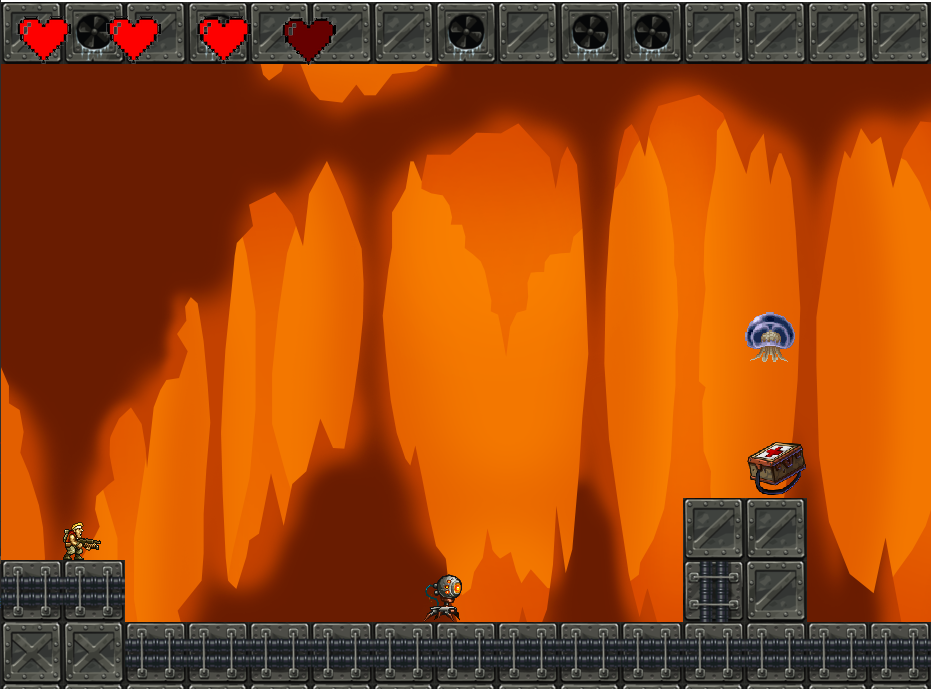
\includegraphics[scale=0.50]{imagenes/EjemploEscena_1.png}
	\caption{\label{fig:EjemploEscena_1}Ejemplo de la fase 1}
\end{figure}

\subsubsection{Fase 2 - Almacen}
En esta segunda escena el protagonista se encuentra con 3 vidas en el almacén, donde tendrá que recoger todas las herramientas (un total de 11) que se va a ir encontrando para completar con éxito esta etapa, también se encontrará con botiquines que le permitirán recuperar vidas, las cuales le podrán ser arrebatadas por los enemigos que entorpecerán su camino, tendrá que hacer frente a 7 tortugas, 6 spiderbots y 7 octopus. Si continúa andando al llegar al final del escenario, pasará a la escena 3. En la Figura \ref{fig:EjemploEscena_2} presenta un ejemplo de la misma. 

\begin{figure}[H]
    \centering
    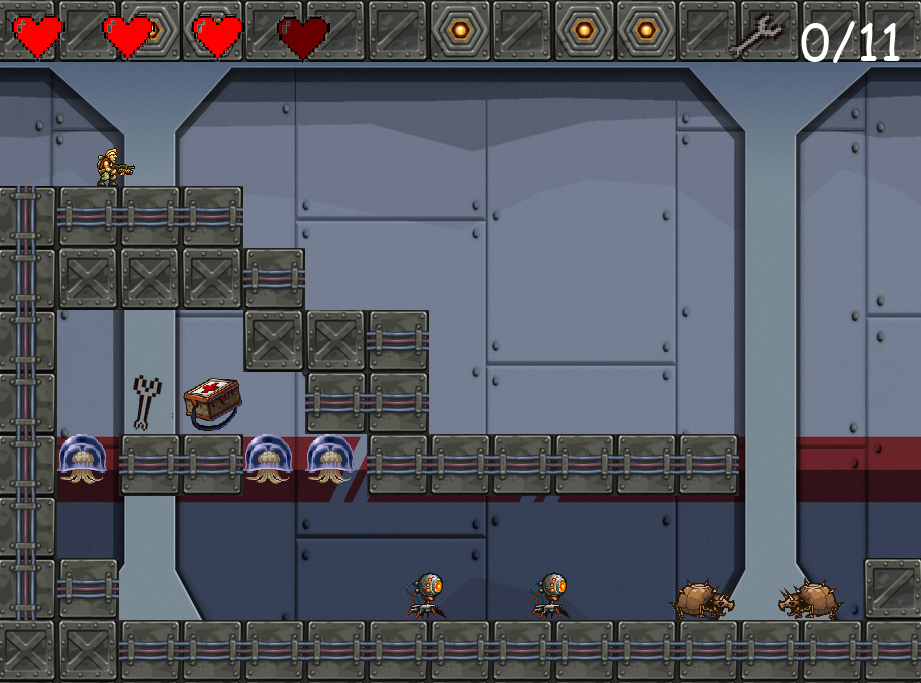
\includegraphics[scale=0.50]{imagenes/EjemploEscena_2.png}
    \caption{\label{fig:EjemploEscena_2}Ejemplo de la fase 2}
\end{figure}
\subsubsection{Fase 3 - Puente de mando de la nave}

En la tercera y última escena el jugador aparece en el Puente de mando con 3 vidas, al igual que en las escenas anteriores, debe llegar al final del escenario con vida intentando destruir a los enemigos que se encuentre a su paso, un total de 20: 7 tortugas, 7 octopus y 6 spiderbots. Si consigue llegar con vida al final de esta escena habrá completado la aventura y llegará a la pantalla de Victoria. En la Figura \ref{fig:EjemploEscena_3} presenta un ejemplo de la misma.

\begin{figure}[H]
    \centering
    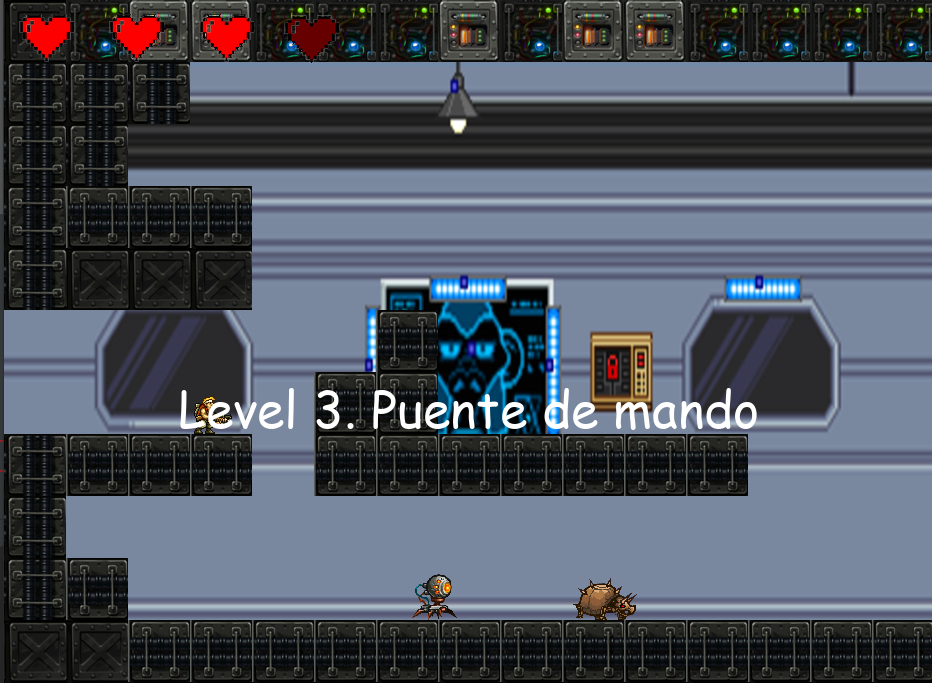
\includegraphics[scale=0.50]{imagenes/EjemploEscena_3.png}
    \caption{\label{fig:EjemploEscena_3}Ejemplo de la fase 3}
\end{figure}

\subsubsection{Créditos}
Pantalla en la que se visualiza la lista de nombres de los desarrolladores y del product owner. Desde esta pantalla se permite al jugador volver al menú principal pulsando la tecla Esc. Ejemplo en la Figura \ref{fig:EjemploCreditos}.

\begin{figure}[H]
	\centering
	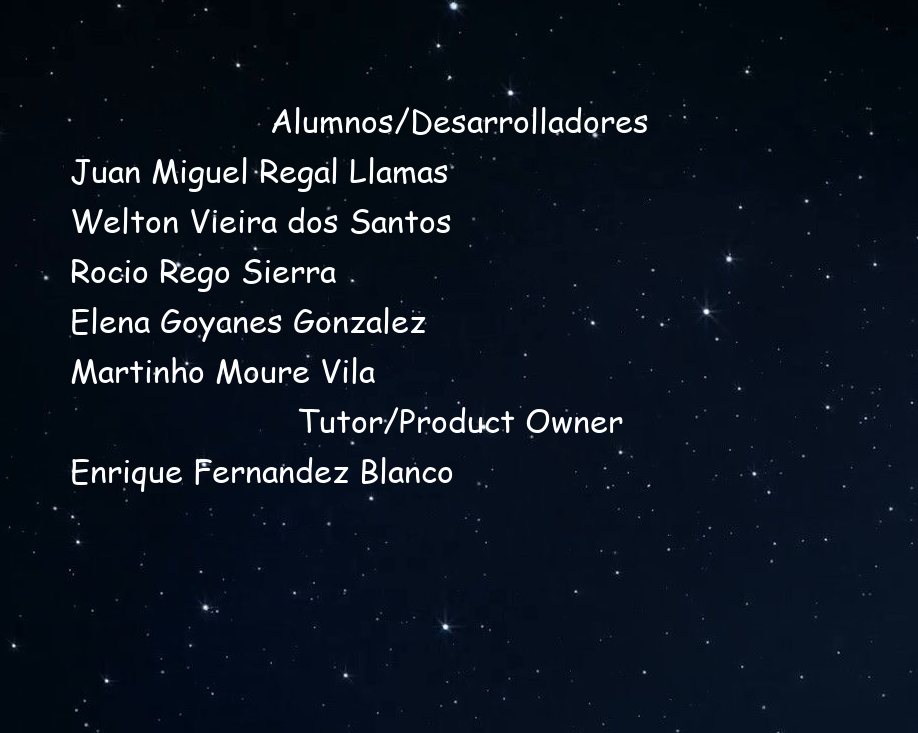
\includegraphics[scale=0.50]{imagenes/ApartadoCreditos.png}
	\caption{\label{fig:EjemploCreditos}Ejemplo del apartado créditos del menú principal}
\end{figure}

\subsubsection{Victoria}
En esta pantalla se muestra un aviso de que el jugador ha conseguido ganar y terminar el juego. Para volver al menú principal se puede pulsar la tecla Esc. Ejemplo en la Figura \ref{fig:EjemploVictoria}.

\begin{figure}[H]
	\centering
	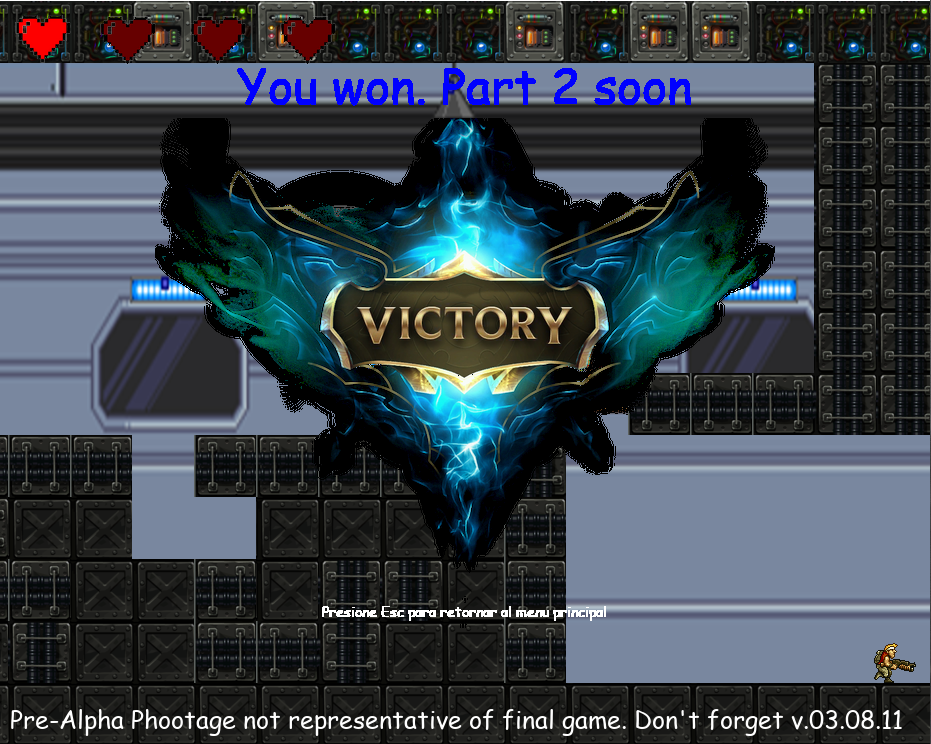
\includegraphics[scale=0.50]{imagenes/victoria.png}
	\caption{\label{fig:EjemploVictoria}Ejemplo de la escena de victoria}
\end{figure}

\subsubsection{Derrota}
Aquí se informa al jugador de que ha sido derrotado, tras haberse quedado sin vidas. Desde esta pantalla se puede volver al menú principal pulsando a tecla Esc. Ejemplo en la Figura \ref{fig:EjemploDerrota}.

\begin{figure}[H]
	\centering
	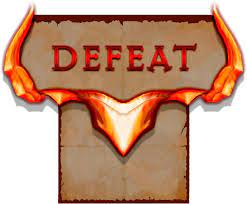
\includegraphics[scale=0.60]{imagenes/derrota.png}
	\caption{\label{fig:EjemploDerrota}Ejemplo de la escena de derrota}
\end{figure}

\subsubsection{Pausa}
Aquí se informa al jugador de que el juego sido pausado despues de precionar la tecla de escape (esc). Desde esta pantalla se puede volver al menú principal pulsando a tecla Esc o seleccionar la opción \textbf{Menu Principal}. Ejemplo en la Figura \ref{fig:EjemploPausa}.

\begin{figure}[H]
	\centering
	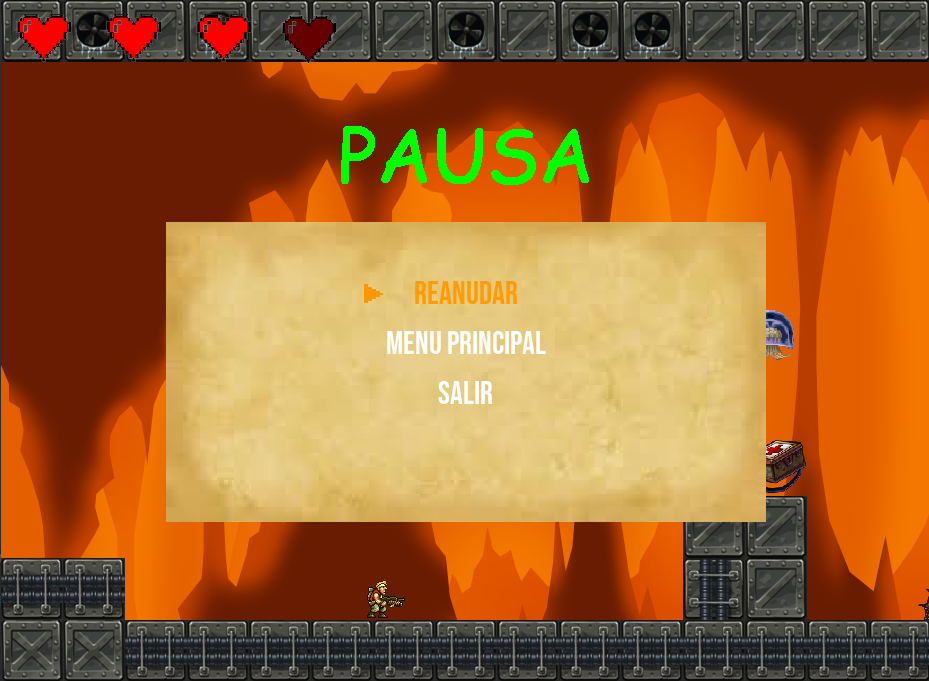
\includegraphics[scale=0.50]{imagenes/Pausa.png}
	\caption{\label{fig:EjemploPausa}Ejemplo de pausar el juego}
\end{figure}

\subsection{Aspectos destacables y detalles de su implementación}

\subsubsection{Creacción de las fases}
Un aspecto del proyecto que cabe destacar es la forma en que se crean los escenarios y se posicionan los enemigos e items, esta parte se realiza a través de una arquitectura dirigida por datos, donde cada escenario está representado por una matriz de números en un fichero .txt, donde cada número representa un tipo de bloque diferente y los ceros que no hay ningún bloque. 

Los tipos de bloque (“tiles”) están representados en ficheros json, con un array de elementos, cada uno con un identificador que corresponde al valor numérico en la matriz. El nombre de la hoja de sprites que contiene el sprite del bloque y la posición en la hoja de sprites. 

La colocación de los enemigos y los items es parecida:  

Para cada enemigo y para cada item tenemos un fichero json formado por un array de elementos. Estos elementos contienen un nº identificador, la posición en el eje x y la posición en el eje y. 

Después estos datos son leídos por las funciones: 

“readMatrix” : Para leer a matriz que representa o escenario 

“readPosition”: Para leer de las posiciones de los items y los enemigos 

“ReadTileReferences”: para leer o json que define los bloques (“tiles”) 

\subsubsection{Dinámicas de ataques}

Tanto para los disparos del personaje, como para los enemigos y los items, para que no se crearan y destruyeran objetos de forma que acabara pasando el recolector de basura provocando que se atasque el juego, todos estos elementos son creados al iniciarse el nivel, y al tener que ser destruidos son cambiados del grupo al que corresponden a un grupo que no se actualiza, por lo que se mantienen sus referencias de modo que el juego no se atasca borrandolos, pero tampoco se pierde tiempo de ejecución actualizándolos. 

Para los disparos, creamos un array de un nº máximo de balas suficientes para que se puedan reutilizar sin que el jugador se entere, este array pertenece al personaje que las dispara y sus balas al inicializarse pertenecerán al grupo de balas que no se actualizan, así, cada vez que dispare llamará a una función que le reinicia todos los atributos a la bala y esta se añade al grupo de balas que sí se actualizan. 

En el protagonista al disparar se calculará el ángulo de disparo del ratón respecto al protagonista. 

\section{Videojuego en 3D}

\subsection{Descripción}
ISS Manticore 3D es un First Person Shooter(FPS), donde el protagonista debe superar diferentes desafios hasta alcanzar su objetivo. Para ello dispondrá de armamento del que se podrá ayudar para derrotar a los distintos enemigos que tratarán de entorpecer su paso. Al comienzo de la aventura tendrá que desplazarse hasta encontrar las dos palancas que le permitiran pasar a la siguiente fase, durante este trayecto tendrá que eliminar a todos los enemigos que se crucen en su camino. Una vez completado este desafio, el personaje tendrá que arreglar un genarador, para ello ha de permanecer en la zona en que se encuentra el motor durante un tiempo suficiente, esto no va a resultarle tarea fácil puesto que habrá multiples enemigos tratando de dañarlo. Finalmente tendrá que conseguir llegar a una pequeña nave de emergencia, ayudandose de su gancho para ir avanzando por cajas u otros objetos que se encontrará por el espacio y le permitirán alcanzar la nave. 

\subsubsection{Personajes}

En esta entrega 3D, solamente tendrá un personaje principal, es decir, el mismo aventurero y cariñoso Jackie.

Como en la entrega 2D, el protagonista tendrá que completar distintas fases, en las que tendrá que superar distintos enemigos y acometer distintas tareas para alcanzar su objetivo, para ello el jugador tendrá que mover al protagonista empleando las flechas del teclado para avanzar, esquivar a los enemigos y recoger los coleccionables necesarios y disparando con un click de ratón a los distintos personajes que se interpongan en su camino. La dinámica es la misma con excepción de que ahora se pondrá acompañar el personaje en primera persona y el manejo de la visón de jack se efectuará desde el ratón.

\subsubsection{Enemigos}

\subsection{Escenas}

La transición entre escenas se muestra en el diagrama de la Figura \ref{fig:TrasicionEscenas3D}. 

\begin{figure}[H]
	\centering
	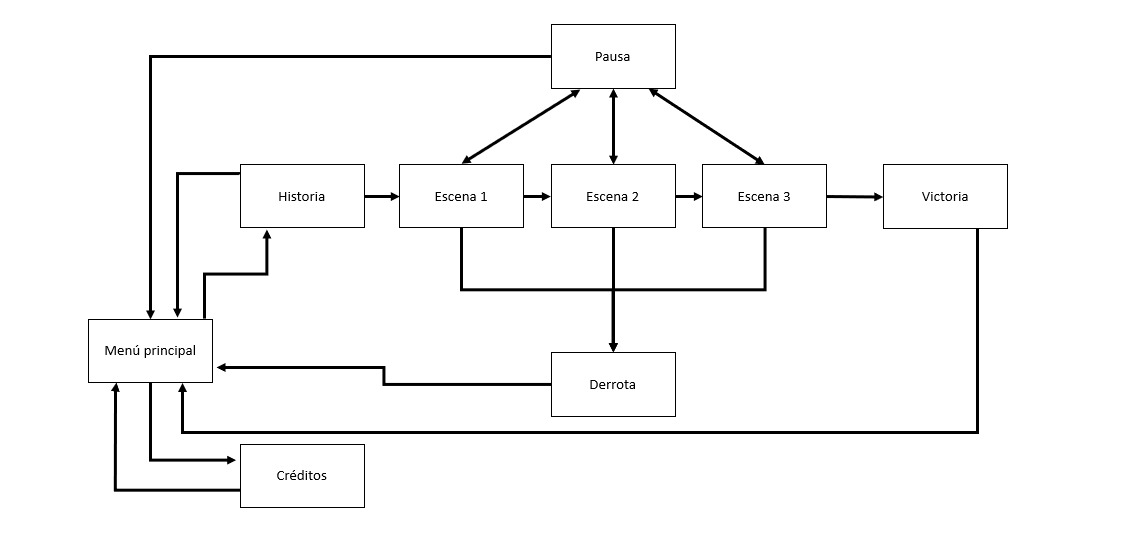
\includegraphics[scale=0.35]{imagenes/transicionEscenas.jpeg}
	\caption{\label{fig:TrasicionEscenas3D}Diagrama de transición de las escenas}
\end{figure}

\subsubsection{Escena 1}
La primera fase empieza en un extremo del escenario donde el personaje tiene que ir avanzando e ir completando los retos que ese escenario va proponiendo.

La única forma de superar esa fase es eliminando todos los enemigos y accionar dos palancas, que estan distribuidas por el escenario, para abrir una puerta y dar paso a la segunda fase.

Para el diseño de este escenario se han utilizado los Prefabs que proporcionan los siguientes paquetes:
\begin{itemize}
	\item paquete Prefab 1: kdjsflksdfkljaklfjalfa
	\item Prefab 2: kdjsflksdfkljaklfjalfa
	\item Prefab 3: kdjsflksdfkljaklfjalfa
	\item Prefab 4: kdjsflksdfkljaklfjalfa
\end{itemize}

\subsubsection{Escena 2}
La segunda fase se empieza también es un extremo del escenario y para superarla será necesario superar los retos que se presenten de la misma forma que la fase anterior.

Para completar esa fase, es necesario arreglar un “generador” que se encuentra en el centro del escenario que, posiblemente estará plagado de enemigos que intentarán imposibilitar que el personaje principal arregle el problema en dicho equipo eléctrico. Para solucionar el problema, el personaje simplemente tendrá que estar cerca de él durante un tiempo mientras se carga el porcentaje visible en pantalla. Una vez se complete, el generador tendrá su problema resuelto y el personaje tendrá que volver por el mismo camino por el cual llegó para pasar a la última fase.

Para el diseño de este escenario se han utilizado los Prefabs que proporcionan los siguientes paquetes:
\begin{itemize}
	\item paquete Prefab 1: kdjsflksdfkljaklfjalfa
	\item Prefab 2: kdjsflksdfkljaklfjalfa
	\item Prefab 3: kdjsflksdfkljaklfjalfa
	\item Prefab 4: kdjsflksdfkljaklfjalfa
\end{itemize}

\subsubsection{Escena 3}
En la tercera fase, como en las anteriores, el personaje empieza en un extremo de la misma y va avanzando dentro de esa escena.

El objetivo es huir de esa nave para llegar a otra pequeña nave de emergencia que se encuentra localizada en el otro extremo de ese escenario. El único inconveniente que el personaje va encontrar es que él mismo tiene que buscar una forma de acceder a dicha nave de emergencia, que está localizada en un plano distinto al del protagonista.

El personaje encontrará cajas flotantes que él mismo podrá escalar directamente o utilizar un recurso de ``gancho'' especial para porder escalar. Una vez llegado al objetivo, el personaje entrará en dicha nave de emergencia y esa fase se dará por concluida.

Para el diseño de este escenario se han utilizado los Prefabs que proporcionan los siguientes paquetes:
\begin{itemize}
	\item paquete Prefab 1: kdjsflksdfkljaklfjalfa
	\item Prefab 2: kdjsflksdfkljaklfjalfa
	\item Prefab 3: kdjsflksdfkljaklfjalfa
	\item Prefab 4: kdjsflksdfkljaklfjalfa
\end{itemize}

\subsection{Aspectos destacables y detalles de su implementación}

\subsubsection{Controlador del personaje}
El personaje se controla desde una perspectiva en primera persona. Como base del controlador,  se hace uso del ``Asset tal'' que se encuetra en la carpeta tal.

Originalmente el personaje tenia un comportamiento tal.....

Se modifica el controlador en ``Eso'' para lograr una adaptación ``tal'' para funcionara con el desarrollo del proyecto actual. Los detalles se lista a continuación:

\begin{itemize}
	\item Movimiento: kldjfalkjdlkjfla
	\item Ataque: dkfñlakflñadskfal
	\item Modo de combate: fkdsjflkajsldj
	\item Rodar: askdjfalksfdjlska
	\item Saltar: lfkjadslkfjaklsdfj
	\item Animaciones: fkjdsfklajflk
\end{itemize}

La mayoría de las animaciones que proporciona el personaje es .........

\subsection{Diseño}

\subsubsection{Diseño del controlador}

\subsubsection{Diseño del HUD - Patrón Observador}

\subsubsection{Diseño de las escenas}

\subsubsection{Camera controler}

\subsubsection{Enemigos - Patrón estrategia}

\subsubsection{Combate - Patrón estrategia}

\subsubsection{Puntuación}

\subsubsection{Menu principal}






